\documentclass[11pt,a4paper]{article}
\usepackage[margin=2.2cm]{geometry}
\usepackage[T1]{fontenc}
\usepackage[utf8]{inputenc}
\usepackage{lmodern}
\usepackage{microtype}
\usepackage{amsmath,amssymb}
\usepackage{booktabs}
\usepackage{array}
\usepackage{multirow}
\usepackage{enumitem}
\usepackage{caption}
\usepackage{subcaption}
\usepackage{xcolor}
\usepackage{tikz}
\usetikzlibrary{arrows.meta,positioning,calc,fit,backgrounds}
\usepackage{pgfplots}
\usepackage{pgfplotstable}
\pgfplotsset{compat=1.17}
\usepackage[hidelinks]{hyperref}

\definecolor{cours}{HTML}{3B6EA8}
\definecolor{cludvig}{HTML}{E08A2E}
\definecolor{coccam}{HTML}{3D9A6B}
\definecolor{cgrey}{HTML}{777777}
\newcommand{\hit}{\textcolor{coccam}{$\bullet$}}
\newcommand{\miss}{\textcolor{cgrey}{$\circ$}}
\newcommand{\code}[1]{\texttt{\small #1}}
\makeatletter\newcommand{\inputtable}[1]{\@@input #1 }\makeatother   % \input that works after \\ inside tabular

\title{\textbf{Training-free lift baselines}\\[2pt]
\large The original LUDVIG and Occam's LGS code against our lift, on backroom and flightroom}
\author{Radiance FYP --- semantic embedding\\ \small intellisense08 (RTX 2080, 8\,GB), 13 October 2026}
\date{}

\begin{document}
\maketitle

\begin{abstract}
\noindent We ran the authors' own code for two training-free lifting methods, LUDVIG (naver/ludvig, ICCV 2025) and
Occam's LGS (insait-institute/OccamLGS), on our two scenes. We gave them exactly our Gaussians, our refined training
cameras and our cached CLIP and DINOv2 teacher maps, and scored the resulting per-Gaussian tables with our unchanged
query and evaluator. This isolates the lift from everything else. \textbf{LUDVIG's lift reproduces ours to numerical
precision} (feature cosine 1.0000 on every Gaussian), so it scores identically. \textbf{Occam's centre-pixel lift is
6--18$\times$ faster} and agrees closely (CLIP cosine median 0.997). It finds the same number of objects with the
multi-scale teachers (22/29) and one more with the scale-averaged teachers (21 vs 20/29). On 29 queries none of these
differences is significant. The lift is not the bottleneck; the 2D teachers and the query are.
\end{abstract}

\tableofcontents
\bigskip

% ─────────────────────────────────────────────────────────────────────────────
\section{Key findings}
\begin{enumerate}[leftmargin=*,itemsep=2pt]
  \item \textbf{Our lift is LUDVIG's lift.} Using LUDVIG's CUDA kernel on the Inria rasteriser, every Gaussian's CLIP,
        DINO and per-scale CLIP row has cosine 1.0000 with ours on both scenes. The seen sets differ by at most one
        Gaussian. Hits, errors and peaks are identical on every query (\S\ref{sec:verify}, \S\ref{sec:results}). Our
        gradient-based implementation is a faithful, independently verified implementation of LUDVIG eq.~3.
  \item \textbf{Occam's LGS gives nearly the same tables, much faster.} It samples the feature only at the pixel under
        each Gaussian's projected centre. CLIP rows agree with ours to a median cosine of 0.997 and DINO rows to 0.98.
        It leaves 4.8\,\% (backroom) and 7.3\,\% (flightroom) of the Gaussians unseen, against 0.1--0.4\,\% for the
        all-pixel lift. It lifts the scale-averaged teachers in 28\,s and 38\,s, against our 181\,s and 262\,s.
  \item \textbf{Localisation is unchanged within noise.} With the multi-scale teachers (A) all three methods hit 22/29.
        With the scale-averaged teachers (Old), Occam's hits 21/29 against 20/29 (one flightroom query). With DINO at
        query time (L-CD), Occam's loses 1--2 queries. Every difference is $\leq 2$ of 29 queries, well inside the noise
        of this set.
  \item \textbf{Consequence for the project.} The lift is settled. All-pixel and centre-pixel lifting both work, and
        the choice between them is about cost, not accuracy. Improvements have to come from the 2D teachers and the
        query: floor calibration, scale and region choice, recognition. Occam's speed makes it cheap to lift many
        more teacher maps, for example more scale groups or SAM levels, which is useful for \code{semantic/new}.
\end{enumerate}

% ─────────────────────────────────────────────────────────────────────────────
\section{What was compared}
\subsection{The three lifts}
All three give each Gaussian $i$ a feature from the 2D teacher maps $F_v$ of the training views $v$, weighted by the
Gaussian's alpha-blending weight $w_i(v,p)=\alpha_i(v,p)\prod_{j<i}(1-\alpha_j(v,p))$.

\begin{description}[leftmargin=1.2em,style=nextline]
  \item[Ours (\code{radiance\_semantics/lift.py}, gsplat 1.0.0)]
    $\displaystyle f_i=\frac{\sum_{v,p} w_i(v,p)\,F_v(p)}{\sum_{v,p} w_i(v,p)}$ over \emph{every pixel}. The numerator
    is the gradient of $\sum_p\langle\mathrm{render}(f),F_v\rangle$ at $f=0$ and the denominator the gradient of
    $\sum_p \mathrm{render}(\mathbf 1)$: two backward passes in 32-channel chunks (gsplat's backward limit).
  \item[LUDVIG (original code)] The same equation (paper eq.~3, $f=D^{-1}W^\top F$), computed by a dedicated CUDA
    kernel (\code{apply\_weights}) inside the Inria rasteriser. It accumulates $w\,F$ and $w$ in one forward pass.
  \item[Occam's LGS (original code)] The maximum-likelihood estimate simplified to the \emph{centre pixel} (paper
    eq.~7): $\displaystyle f_i=\frac{\sum_{v} w_i^v\,F_v(\lfloor x_i'^v\rfloor)}{\sum_v w_i^v}$, where $x_i'^v$ is the
    projected centre and $w_i^v$ the blend weight at that pixel, recorded by their gsplat 1.4.0 fork during an ordinary
    forward render. Gaussians never blended at their centre pixel are dropped ("filtering").
\end{description}

\subsection{Controlled design}
Only the lift changes. Figure~\ref{fig:design} shows the data flow.
\begin{itemize}[leftmargin=*,itemsep=1pt]
  \item \textbf{Same inputs.} \code{export\_scene.py} (kitchen env) writes the trained splatfacto Gaussians in the
        Inria PLY layout, in checkpoint order, together with the 270 / 450 training views our lift uses: refined
        SO3$\times$R3 poses, pose outliers dropped, centred principal points. Both runners read our cached teacher
        grids and upsample them to the 960\,px render exactly as our lift does (bilinear, \code{align\_corners=False}).
  \item \textbf{Original code.} Each method runs in its own conda env (\code{ludvig}: torch 2.4.0; \code{occamlgs}: torch
        2.2.2 with their gsplat fork; both cu118 built for sm\_75), never in kitchen. The runners call the papers'
        functions: \code{GaussianModel.apply\_weights}; \code{gaussian\_renderer.render} plus
        \code{accumulate\_gaussian\_feature\_per\_view}.
  \item \textbf{Same scoring.} The runners write \code{lift<suffix>\_raw/} in our lift step's layout. Our own
        \code{export} step builds the table in \code{.splat} order, and our unchanged evaluator scores it with the
        Phase~1 query settings (floor 0.55, $\tau=0.55+0.5(\text{peak}-0.55)$, 0.1\,m voxels, $\geq$15 Gaussians).
  \item \textbf{Teachers.} Old = OpenCLIP ViT-B/16 7-scale pyramid, scales averaged (\code{d7a30d7264}). A =
        the same crops kept in three scale groups, the group chosen per query (\code{9c437cce68}, our default since
        8 Oct). DINOv2 ViT-S/14 for the DINO rows.
  \item \textbf{Query sets.} The Phase~5 sets frozen on 6 Oct (backroom amended 7 Oct): 13 + 16 = 29 positives and
        3 + 3 = 6 absent objects. They were not used to tune anything here. The Phase~1 development set (5 backroom
        queries) served as a first check.
\end{itemize}

\begin{figure}[t]
\centering
\resizebox{\linewidth}{!}{%
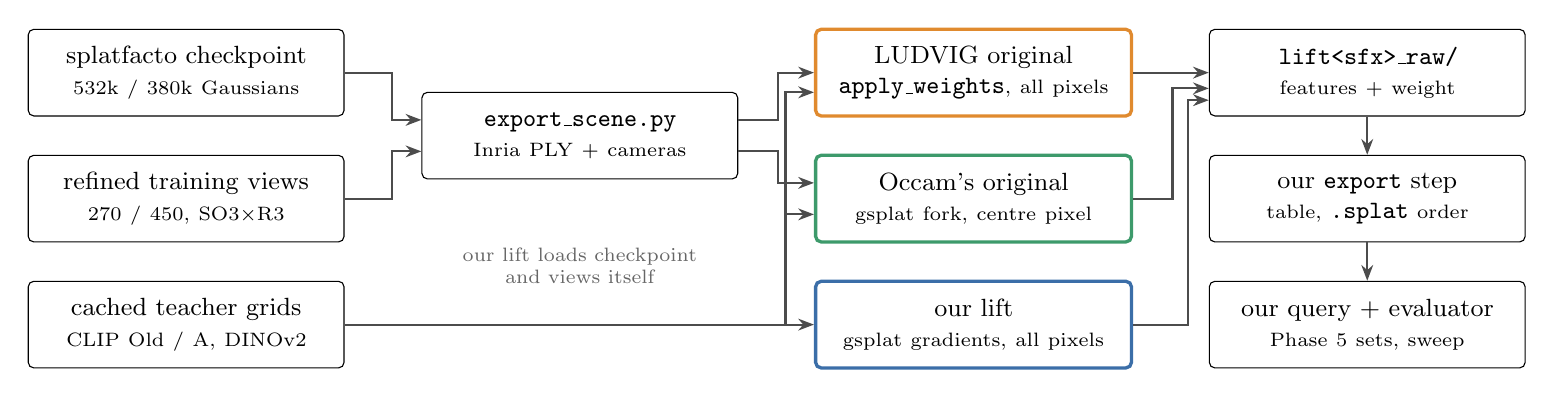
\begin{tikzpicture}[font=\small,
  box/.style={draw, rounded corners=2pt, align=center, minimum height=11mm, text width=38mm, inner sep=3pt, fill=white},
  ours/.style={box, draw=cours, very thick}, lud/.style={box, draw=cludvig, very thick}, occ/.style={box, draw=coccam, very thick},
  arr/.style={-{Stealth[length=2mm]}, thick, draw=black!70}]
  % column 1: shared inputs
  \node[box] (ck)  at (0, 0)    {splatfacto checkpoint\\\scriptsize 532k / 380k Gaussians};
  \node[box] (cam) at (0,-1.6)  {refined training views\\\scriptsize 270 / 450, SO3$\times$R3};
  \node[box] (tea) at (0,-3.2)  {cached teacher grids\\\scriptsize CLIP Old / A, DINOv2};
  % column 2: export for the originals
  \node[box] (exp) at (5.0,-0.8) {\code{export\_scene.py}\\\scriptsize Inria PLY + cameras};
  % column 3: the three lifts
  \node[lud]  (lud)  at (10.0, 0)    {LUDVIG original\\\scriptsize \code{apply\_weights}, all pixels};
  \node[occ]  (occ)  at (10.0,-1.6)  {Occam's original\\\scriptsize gsplat fork, centre pixel};
  \node[ours] (lift) at (10.0,-3.2)  {our lift\\\scriptsize gsplat gradients, all pixels};
  % column 4: shared scoring
  \node[box] (raw) at (15.0, 0)    {\code{lift<sfx>\_raw/}\\\scriptsize features + weight};
  \node[box] (tab) at (15.0,-1.6)  {our \code{export} step\\\scriptsize table, \code{.splat} order};
  \node[box] (ev)  at (15.0,-3.2)  {our query + evaluator\\\scriptsize Phase 5 sets, sweep};
  % arrows
    \draw[arr] (ck.east) -- ++(0.6,0) |- ([yshift=2mm]exp.west);
  \draw[arr] (cam.east) -- ++(0.6,0) |- ([yshift=-2mm]exp.west);
  \draw[arr] ([yshift=2mm]exp.east) -- ++(0.5,0) |- (lud.west);
  \draw[arr] ([yshift=-2mm]exp.east) -- ++(0.5,0) |- ([yshift=2mm]occ.west);
  \draw[arr] (tea.east) -- (lift.west);
  \draw[arr] (tea.east) -- ++(5.6,0) |- ([yshift=-2mm]occ.west);
  \draw[arr] (tea.east) -- ++(5.6,0) |- ([yshift=-2.5mm]lud.west);
  \draw[arr] (lud.east) -- (raw.west);
  \draw[arr] (occ.east) -- ++(0.5,0) |- ([yshift=-2mm]raw.west);
  \draw[arr] (lift.east) -- ++(0.7,0) |- ([yshift=-3.5mm]raw.west);
  \draw[arr] (raw) -- (tab); \draw[arr] (tab) -- (ev);
  \node[font=\scriptsize, text=black!60, align=center] at (5.0,-2.45) {our lift loads checkpoint\\and views itself};
\end{tikzpicture}}
\caption{Controlled comparison. Gaussians, cameras and teacher maps are shared. Only the lift differs (blue: ours;
orange: LUDVIG; green: Occam's LGS, both the authors' own code). Table building, query and evaluation are ours and
unchanged.}
\label{fig:design}
\end{figure}

\subsection{Adaptations needed to run the original code}
\begin{itemize}[leftmargin=*,itemsep=1pt]
  \item \textbf{No pruning.} LUDVIG optionally keeps the top-$k$ Gaussians by total weight, and Occam's removes
        never-activated Gaussians. We keep every row and give dropped Gaussians weight 0. To the query this is the
        same thing (it ignores unseen rows), and table rows must stay aligned with the \code{.splat} file.
  \item \textbf{LUDVIG's weight count.} The kernel adds $\alpha T$ to the weight counter once per \emph{channel} (inside
        its channel loop), so its normaliser is $C\cdot\sum w$. In LUDVIG's own pipeline this scales every feature by
        $1/C$, which normalisation removes. We divide it out to store the true blend weight. The kernel is compiled
        for fixed channel counts, so our 384-d DINO is lifted in chunks of 256 + 100 + 20 + 3 + 3 + 2.
  \item \textbf{Occam's teacher mask.} Occam's code multiplies by LangSplat's validity mask. Our teacher maps cover
        every pixel, so the mask is all ones.
  \item \textbf{Rasteriser differences} (inherent to the originals, kept): the Inria rasteriser culls Gaussians
        within 0.2\,m of the camera and clamps $\alpha\le0.99$; gsplat uses its own near plane. Both assume a centred
        principal point, which holds exactly on our scenes. Lens distortion is ignored by all three methods alike.
\end{itemize}

% ─────────────────────────────────────────────────────────────────────────────
\section{Verification: how close are the tables?}\label{sec:verify}
\code{table\_agreement.py} compares every Gaussian seen by both tables. Rows are unit length, so the cosine is the
dot product. Table~\ref{tab:agree} and Figure~\ref{fig:agree} give the results.

\begin{table}[h]
\centering\small
\caption{Per-Gaussian agreement with our lift (Gaussians seen by both). Median cosine, 1st-percentile cosine, and the
share of rows with cosine $>0.99$.}
\label{tab:agree}
\begin{tabular}{llcccccc}
\toprule
& & \multicolumn{3}{c}{backroom} & \multicolumn{3}{c}{flightroom}\\
\cmidrule(lr){3-5}\cmidrule(lr){6-8}
Pair & Feature & median & p1 & $>0.99$ (\%) & median & p1 & $>0.99$ (\%)\\
\midrule
\inputtable{tables/agreement.tex}
\bottomrule
\end{tabular}
\end{table}

\begin{figure}[h]
\centering
\begin{tikzpicture}
\begin{axis}[width=0.85\linewidth, height=5.2cm, ymode=log, ymin=1e-5, ymax=1, xmin=0, xmax=1,
  xlabel={cosine with our lift (per Gaussian)}, ylabel={share of Gaussians},
  legend pos=north west, legend style={font=\scriptsize}, grid=major, grid style={gray!20}]
  \addplot[const plot mark mid, thick, black] table[x=bin, y=br_clip, col sep=comma] {data/agreement_hist.csv};
  \addplot[const plot mark mid, thick, black, dashed] table[x=bin, y=br_dino, col sep=comma] {data/agreement_hist.csv};
  \addplot[const plot mark mid, thick, violet] table[x=bin, y=fr_clip, col sep=comma] {data/agreement_hist.csv};
  \addplot[const plot mark mid, thick, violet, dashed] table[x=bin, y=fr_dino, col sep=comma] {data/agreement_hist.csv};
  \legend{backroom CLIP, backroom DINO, flightroom CLIP, flightroom DINO}
\end{axis}
\end{tikzpicture}
\caption{Occam's LGS vs our lift, Old teachers: distribution of per-Gaussian cosine (log scale). LUDVIG is not shown:
every one of its rows has cosine 1.0000 with ours.}
\label{fig:agree}
\end{figure}

\paragraph{Reading.} LUDVIG's kernel and our gradient trick compute the same sum, so the tables agree to float
precision. Occam's rows are a single-pixel sample per view instead of a footprint average, so they differ slightly.
CLIP differs least, because our CLIP teacher grid ($\approx71\times40$ cells) is smooth at Gaussian scale and the
centre pixel sees nearly the footprint's average. DINO differs more: its grid is similarly coarse, but neighbouring
DINO cells differ more. A 3-view spot check before the full runs showed the same pattern (CLIP p1 0.958, DINO p1 0.75),
and every Gaussian Occam's activated was also seen by our lift.

% ─────────────────────────────────────────────────────────────────────────────
\section{Results on the Phase 5 sets}\label{sec:results}

\begin{table}[h]
\centering\small
\caption{Phase 5 evaluation, top-1 hits per scene and combined (29 positives), median localisation error of the
returned candidates, absent objects that returned a candidate (of 3 per scene), and AUROC of peak relevancy
(positives vs absent). Query settings unchanged from Phase 1.}
\label{tab:summary}
\setlength{\tabcolsep}{4pt}
\begin{tabular}{llc cccc cccc}
\toprule
& & & \multicolumn{4}{c}{backroom (13 + 3)} & \multicolumn{4}{c}{flightroom (16 + 3)}\\
\cmidrule(lr){4-7}\cmidrule(lr){8-11}
Lift & Teach. & Total & hits & err (m) & FP & AUROC & hits & err (m) & FP & AUROC\\
\inputtable{tables/summary.tex}
\bottomrule
\end{tabular}
\end{table}

\begin{figure}[h]
\centering
\begin{tikzpicture}
\begin{axis}[ybar, width=0.9\linewidth, height=5.5cm, bar width=9pt, ymin=15, ymax=25,
  symbolic x coords={Ours,LUDVIG,Occam}, xtick=data, enlarge x limits=0.25,
  ylabel={top-1 hits (of 29)}, legend style={at={(0.5,1.03)}, anchor=south, legend columns=4, font=\scriptsize},
  nodes near coords, every node near coord/.append style={font=\tiny}, grid=major, grid style={gray!20}]
  \addplot[fill=cours!45, draw=cours] table[x=method, y=OldLC, col sep=comma] {data/hits_bars.csv};
  \addplot[fill=cours, draw=cours] table[x=method, y=ALC, col sep=comma] {data/hits_bars.csv};
  \addplot[fill=black!20, draw=black!60] table[x=method, y=OldLCD, col sep=comma] {data/hits_bars.csv};
  \addplot[fill=black!55, draw=black!70] table[x=method, y=ALCD, col sep=comma] {data/hits_bars.csv};
  \legend{Old L-C, A L-C, Old L-CD, A L-CD}
\end{axis}
\end{tikzpicture}
\caption{Combined top-1 hits on both scenes, by lift method, teachers and query mode (L-C: CLIP relevancy; L-CD: plus
DINO diffusion and split).}
\label{fig:bars}
\end{figure}

\begin{table}[p]
\centering\small
\caption{Per-query outcome, L-C (\hit\ hit, \miss\ miss). Queries in bold differ between methods.}
\label{tab:perquery}
\begin{tabular}{l cccccc}
\toprule
& \multicolumn{3}{c}{Old teachers} & \multicolumn{3}{c}{A teachers}\\
\cmidrule(lr){2-4}\cmidrule(lr){5-7}
Query & Ours & LUDVIG & Occam & Ours & LUDVIG & Occam\\
\inputtable{tables/per_query.tex}
\bottomrule
\end{tabular}
\end{table}

\paragraph{Reading.}
\begin{itemize}[leftmargin=*,itemsep=2pt]
  \item \textbf{LUDVIG = ours, query for query.} The two lifts agree on all 29 positives and 6 absent objects, in both
        query modes and with both teacher sets. Median errors are identical, and the 90th-percentile errors differ by
        at most 1\,mm. Only the query times differ (0.53--3.2\,s), which is CPU noise: the tables hold the same numbers.
  \item \textbf{Occam's LGS: $\pm1$--2 queries, in both directions.} With CLIP alone (L-C), Occam's Old table gains the
        flightroom \emph{armchair} (21 vs 20/29). Occam's A table swaps \emph{office chair} (lost) for \emph{camera tripod}
        (gained, the first hit on this query by any lift or teacher), so it ties at 22/29. With DINO at query time
        (L-CD), Occam's loses \emph{water bottle} (Old, 19/29) and \emph{swivel chair}, \emph{upholstered chair} and
        \emph{water bottle} while gaining \emph{water jug} (A, 20/29). Its DINO rows differ most from the all-pixel
        lift (\S\ref{sec:verify}), and L-CD's diffusion and split use exactly those rows.
  \item \textbf{The teachers move as many queries as the lift, or more.} Going from Old to A changes 3--4 L-C outcomes
        for every lift: \emph{hose reel} is lost, \emph{upholstered chair} and \emph{water jug} are gained, and so is
        \emph{armchair} for ours and LUDVIG's (Occam's already had it with Old). Going from our lift to Occam's on the same
        teachers changes one L-C outcome (Old) or two (A), and one (Old) or four (A) L-CD outcomes. The scale-group
        choice of A recovers the same occluded chairs and the water jug whichever lift produced the table.
  \item \textbf{Localisation.} Occam's median errors are equal or smaller with the Old teachers (0.18 vs 0.19\,m
        backroom, 0.18 vs 0.22\,m flightroom) and mixed with A (0.26 vs 0.21\,m backroom, 0.18 vs 0.25\,m flightroom).
        Backroom A has two "bad position" misses with Occam's against one with ours.
  \item \textbf{Absent objects.} AUROC is equal or higher with Occam's (flightroom 0.917 vs 0.896). At floor 0.55,
        however, Occam's A table fires on both \emph{bicycle} and \emph{ceiling fan} in backroom (2/3 vs 1/3). With the Old
        teachers, sampling one pixel instead of averaging the footprint raises peaks slightly (dev-set peaks +0.003 to
        +0.018), absent objects included; with A the shifts are mixed ($-0.010$ to $+0.012$).
\end{itemize}


\subsection{Development set}
On the 5 backroom development queries (Phase~1 gate) our and LUDVIG's tables hit 5/5 with identical peaks, and
Occam's hit 4/5 (Table~\ref{tab:dev}). With the Old teachers Occam's \emph{garden cart} candidate is a small cluster
(81 Gaussians against our 94) whose centroid lands 0.99\,m from the annotation. With A, \emph{green foam mats} picks a
mat-like region 2.9\,m away. Both are threshold-edge cases of the cluster rules, not systematic failures. The frozen
sets (above) are the evaluation.
\begin{table}[h]
\centering\small
\caption{Development set (5 backroom queries, \code{phase1\_gate}): hits, median error and peak relevancy per query.}
\label{tab:dev}
\begin{tabular}{lccl}
\toprule
Lift, teachers & hits & err (m) & peak relevancy per query$^\dagger$\\
\midrule
\inputtable{tables/dev.tex}
\bottomrule
\multicolumn{4}{l}{\scriptsize $^\dagger$ red tool chest, shop vacuum, green foam mats, garden cart, whiteboard}
\end{tabular}
\end{table}

% ─────────────────────────────────────────────────────────────────────────────
\section{Floor sweep}\label{sec:sweep}
The relevancy floor (0.55) is the one query setting that matters most (SEMANTICS.md \S13, \S16). Sweeping it shows
whether a lift shifts the relevancy scale, which would make a comparison at one fixed floor unfair. The sweep is
post-hoc on the evaluation sets and is reported as such.

\begin{figure}[h]
\centering
\begin{subfigure}{0.49\linewidth}
\begin{tikzpicture}
\begin{axis}[width=\linewidth, height=5.4cm, xlabel={relevancy floor}, ylabel={top-1 hits (of 29)},
  legend style={font=\tiny, at={(0.5,-0.3)}, anchor=north, legend columns=2}, grid=major, grid style={gray!20}, ymin=14, ymax=26]
  \addplot[cours, thick, mark=*, mark size=1.2pt] table[x=floor, y=Old_hits, col sep=comma] {data/floor_sweep.csv};
  \addplot[cours, thick, dashed, mark=square*, mark size=1.2pt] table[x=floor, y=A_hits, col sep=comma] {data/floor_sweep.csv};
  \addplot[cludvig, thick, mark=*, mark size=0.8pt, mark options={solid}] table[x=floor, y=LUDVIGOld_hits, col sep=comma] {data/floor_sweep.csv};
  \addplot[cludvig, thick, dashed, mark=square*, mark size=0.8pt] table[x=floor, y=LUDVIGA_hits, col sep=comma] {data/floor_sweep.csv};
  \addplot[coccam, thick, mark=triangle*, mark size=1.4pt] table[x=floor, y=OccamOld_hits, col sep=comma] {data/floor_sweep.csv};
  \addplot[coccam, thick, dashed, mark=diamond*, mark size=1.4pt] table[x=floor, y=OccamA_hits, col sep=comma] {data/floor_sweep.csv};
  \legend{Ours Old, Ours A, LUDVIG Old, LUDVIG A, Occam Old, Occam A}
\end{axis}
\end{tikzpicture}
\caption{Hits vs floor.}
\end{subfigure}\hfill
\begin{subfigure}{0.49\linewidth}
\begin{tikzpicture}
\begin{axis}[width=\linewidth, height=5.4cm, xlabel={absent objects with a candidate (of 6)}, ylabel={top-1 hits (of 29)},
  legend style={font=\tiny, at={(0.5,-0.3)}, anchor=north, legend columns=2}, grid=major, grid style={gray!20}, ymin=14, ymax=26, xmin=0.5, xmax=6.5]
  \addplot[cours, thick, mark=*, only marks] table[x=Old_fp, y=Old_hits, col sep=comma] {data/floor_sweep.csv};
  \addplot[cours, thick, mark=square, only marks] table[x=A_fp, y=A_hits, col sep=comma] {data/floor_sweep.csv};
  \addplot[coccam, thick, mark=triangle*, only marks, mark size=2.5pt] table[x=OccamOld_fp, y=OccamOld_hits, col sep=comma] {data/floor_sweep.csv};
  \addplot[coccam, thick, mark=diamond, only marks, mark size=2.5pt] table[x=OccamA_fp, y=OccamA_hits, col sep=comma] {data/floor_sweep.csv};
  \legend{Ours/LUDVIG Old, Ours/LUDVIG A, Occam Old, Occam A}
\end{axis}
\end{tikzpicture}
\caption{Hits vs false positives (each point one floor).}
\end{subfigure}
\caption{Relevancy-floor sweep (floors 0.46--0.60), both scenes combined. LUDVIG's curves lie exactly on ours.}
\label{fig:sweep}
\end{figure}

\paragraph{Reading.} LUDVIG's curves coincide with ours at every floor, as expected from identical tables. Occam's
curves cross ours. Its peaks are slightly higher, so at a given floor it keeps a few more candidates. When the methods
are compared at an equal number of absent objects firing, which is the fair comparison:
\begin{center}\small
\begin{tabular}{lcccc}
\toprule
Absent objects with a candidate (of 6) & 1 & 2 & 3 & 4\\
\midrule
Ours / LUDVIG, Old & 19 & \textbf{23} & 23 & 23\\
Ours / LUDVIG, A   & 19 & 22 & 23 & 23\\
Occam's, Old       & 19 & 21 & \textbf{24} & \textbf{24}\\
Occam's, A         & 19 & 21 & \textbf{24} & \textbf{24}\\
\bottomrule
\end{tabular}
\end{center}
\noindent (best hits over the floors 0.46--0.60 with at most that many absent objects firing). Occam's is ahead by one query
at 3--4 false positives and behind by one or two at 2; at 1 false positive every method finds 19. The ceiling over
all floors is 24/29 for every lift and teacher set, the same ceiling the 8 Oct sweep found for B2. As on 8 Oct, the
same two absent objects keep firing whatever the lift: \emph{ceiling fan} (backroom) at every floor for every table,
and \emph{recycling bin} (flightroom) up to floor 0.55 with the Old teachers and 0.575 with A.
These floors are read off the evaluation set and are optimistic.


% ─────────────────────────────────────────────────────────────────────────────
\section{Cost}\label{sec:cost}
\begin{table}[h]
\centering\small
\caption{Lift cost on the RTX 2080 (960\,px renders): wall time of the lift step, peak GPU memory, and share of
Gaussians seen (weight $>0$). Teacher extraction (31--53\,min) is shared by all and excluded.}
\label{tab:cost}
\begin{tabular}{ll ccc ccc}
\toprule
& & \multicolumn{3}{c}{backroom (532k G., 270 views)} & \multicolumn{3}{c}{flightroom (380k G., 450 views)}\\
\cmidrule(lr){3-5}\cmidrule(lr){6-8}
Lift & Teach. & time (s) & GPU (GB) & seen (\%) & time (s) & GPU (GB) & seen (\%)\\
\midrule
\inputtable{tables/cost.tex}
\bottomrule
\end{tabular}
\end{table}

\begin{figure}[h]
\centering
\begin{tikzpicture}
\begin{axis}[ybar, width=0.95\linewidth, height=5.2cm, bar width=8pt, ymode=log, log origin=infty, ymin=10, ymax=3000,
  symbolic x coords={Ours-Old,LUDVIG-Old,Occam-Old,Ours-A,LUDVIG-A,Occam-A}, xtick=data,
  x tick label style={font=\scriptsize}, ylabel={lift time (s, log)}, legend style={font=\scriptsize, at={(0.02,0.98)}, anchor=north west},
  point meta=rawy, nodes near coords={\pgfmathprintnumber[fixed,precision=0]{\pgfplotspointmeta}},
  every node near coord/.append style={font=\tiny}, grid=major, grid style={gray!20}]
  \addplot[fill=black!25, draw=black!70] table[x=config, y=backroom_s, col sep=comma] {data/cost.csv};
  \addplot[fill=violet!45, draw=violet] table[x=config, y=flightroom_s, col sep=comma] {data/cost.csv};
  \legend{backroom, flightroom}
\end{axis}
\end{tikzpicture}
\caption{Lift wall time per scene (log scale).}
\label{fig:cost}
\end{figure}

\paragraph{Reading.} Occam's centre-pixel lift is the cheapest by far: one forward render per view (no backward
pass), with the feature gathered at one pixel per Gaussian. It lifts all 512 CLIP and 384 DINO channels in
\textbf{28\,s / 38\,s} (Old) and \textbf{124\,s / 74\,s} (A, four maps), 6.5--18$\times$ faster than our
gradient lift (181\,s / 262\,s and 1064\,s / 1364\,s). LUDVIG's kernel is the slowest for wide features (369\,s / 633\,s
for Old). It processes every pixel's full channel vector per Gaussian, and its 512-channel template
likely spills registers on sm\_75. Our A lift stays under 1\,GB of GPU memory because its accumulators live in host RAM; the two originals keep
them on the GPU (2.7--3.4\,GB), which still fits the 8\,GB card. Coverage is the price of Occam's speed: 4.8\,\% and
7.3\,\% of the Gaussians are never blended at their own centre pixel and stay unseen (all-pixel lifts: 0.1\,\% and
0.4\,\%). These are mostly small or occluded Gaussians, which the query's opacity and cluster-size filters largely
ignore anyway. Teacher extraction (31--53\,min per scene) dominates every pipeline.


% ─────────────────────────────────────────────────────────────────────────────
\section{Discussion}
\paragraph{Why the lifts barely matter here.} The Phase~5 diagnostic (SEMANTICS.md \S14) found that lifting into 3D
loses almost nothing: relevancy near an annotated object is 0.007 lower in the table than in the 2D teacher grid. This
experiment confirms it from the other side. Two quite different estimators, a footprint-weighted average over every
pixel and a single-pixel sample per view, produce near-identical tables (CLIP cosine $\geq0.997$ in median) and the
same localisation within $\pm2$ of 29 queries. The CLIP teacher grid is coarse ($\approx71\times40$ cells per image), so
at Gaussian scale it is almost constant across a footprint, and how the footprint is sampled hardly changes the result.
The paper-level claims match this: Occam's LGS reports its estimator as the maximum-likelihood solution under
negligible Gaussian overlap, and LUDVIG reports that further optimisation steps do not improve its features.

\paragraph{Statistical caveat.} 29 positives and 6 absent objects over two scenes. A difference of one or two queries
is not significant (exact sign test on the discordant queries, $p\geq0.6$ for every pair). The development-set result (Occam's 4/5 vs 5/5) is one cluster of
81 Gaussians landing 0.99\,m from the garden cart (Old) and one mat-like region chosen over the green foam mats (A),
both near the edge of the query's cluster rules.

\paragraph{What this means for the next steps.}
\begin{itemize}[leftmargin=*,itemsep=2pt]
  \item \textbf{Keep the all-pixel lift as the reference.} It is LUDVIG's lift, now verified against the authors' code.
        It sees the most Gaussians and averages each one over its whole footprint.
  \item \textbf{Use centre-pixel lifting where speed matters.} At 30--120\,s per scene it makes many more teacher
        maps affordable: more crop-scale groups, SAM levels (B2), or per-query re-lifts. It is a natural building block
        for \code{semantic/new}.
  \item \textbf{Put the effort into the 2D side and the query.} This is where queries are won or lost: the floor
        calibration (HANDOVER \S2.1), per-query scale or region choice, recognition of thin objects (tripod, keyboard,
        floor lamp), and the two persistent "absent" detections.
  \item \textbf{Still to run, the faithful pipelines.} This report isolates the lift. The papers' full pipelines
        differ in more than the lift: LUDVIG's DINOv2 ViT-g features with registers, PCA and logistic-regression graph
        diffusion; Occam's SAM-based LangSplat feature maps. Those are the next comparisons on these branches. LUDVIG's
        diffusion is the part most likely to change outcomes, because our simplified L-CD diffusion changed no hit.
\end{itemize}


% ─────────────────────────────────────────────────────────────────────────────
\section{Reproduction}
Code lives on the branches \code{semantic/LUDVIG} (\code{semantics/baselines/ludvig\_lift.py}) and \code{semantic/LGS}
(\code{semantics/baselines/occam\_lift.py}). Both carry the shared \code{env.sh}, \code{install\_*.sh} and
\code{export\_scene.py}. The original repositories are cloned, unmodified, in \code{\textasciitilde/Radiance/third\_party/}.
{\footnotesize
\begin{verbatim}
bash semantics/baselines/install_ludvig.sh          # one-off: conda env `ludvig`
bash semantics/baselines/install_occamlgs.sh        # one-off: conda env `occamlgs`
source ~/Radiance/figs/figs_env.sh                  # kitchen
python semantics/baselines/export_scene.py --scene backroom
source semantics/baselines/env.sh ludvig
python semantics/baselines/ludvig_lift.py --scene backroom --teachers d7a30d7264 --suffix _ludvigpyr
source semantics/baselines/env.sh occamlgs
python semantics/baselines/occam_lift.py  --scene backroom --teachers 9c437cce68 --suffix _occamms
source ~/Radiance/figs/figs_env.sh
python figs/semantic_pipeline.py --scene backroom --backend lift --table-suffix _occamms \
       --clip-mode scales --only export
python -m radiance_semantics.evaluate --scene backroom --variants L-C@occamms L-CD@occamms
\end{verbatim}
}
Raw results (evaluator JSONs, lift statistics, sweep, agreement, logs) are in \code{../raw/}, derived CSVs in
\code{../csv/}. \code{../scripts/collect.py} and \code{make\_tables.py} regenerate everything this report reads.

\end{document}
